% Translator: Yujun Li 
\chapter{实用方法}
\label{chap:practical_methodology}
成功应用\gls{DL}技术不仅仅需要知道存在哪些算法和解释它们如何工作的原则。
一个好的\gls{ML}实践者也需要知道如何挑选一个针对特别应用的算法,以及如何监管和回应实验中得到的反馈以改进\gls{ML}系统。
在\gls{ML}系统的日常开发中,实践者需要决定是否收集更多的数据,增加或减少模型容量,添加或删除正则化功能,改进模型的优化,改进模型的近似推理,或调试模型的软件实现。
所有这些操作至少都是要费时去尝试的,因此确定正确的做法,而不是盲目猜测是尤为重要的。

本书大部分是关于不同的\gls{ML}模型,训练算法和目标函数。
这可能给人一个印象,成为\gls{ML}专家的最重要因素是了解各种各样的\gls{ML}技术,熟悉各种不同的数学。
在实践中,正确使用一个普通算法通常比草率使用一个不清楚的算法效果更好。
一个算法的正确应用取决于掌握一些相当简单的方法。
本章中的许多建议改编自\cite{ng-lecture-advice}。

我们建议以下几个实用的设计流程:
\begin{itemize}
\item 确定你的目标---使用什么\gls{error_metric},并为此\gls{error_metric}指定目标值。
这些目标和\gls{error_metric}应受驱动于该应用旨在解决的问题。

% -- 409 --

\item 尽快建立一个工作\gls{end_to_end}的流程,包括合适的\gls{performance_metrics}的估计。

\item 搭建好系统以确定性能的瓶颈。
诊断哪个部分的性能差于预期,以及是否因为过拟合,欠拟合,或者数据或软件中的缺陷造成的。

\item 根据系统上的具体观察反复进行逐步变动,如收集新数据,调整超参数,或改变算法。
\end{itemize}

我们将使用街景地址号码\gls{transcription_system}\citep{Goodfellow+et+al-ICLR2014a}作为一个正在运行的示例。
该应用的目标是添加建筑物到谷歌地图。
街景车拍摄建筑物,并记录与每张照片相关的GPS坐标。
\gls{CNN}识别每张照片上的地址号码,由谷歌地图数据库在正确的位置添加该地址。
这个商业应用如何开发的流程是一个很好的如何遵循我们倡导的设计方法的例子。

我们现在描述这个过程中的每一个步骤。

\section{\glsentrytext{performance_metrics}}
\label{sec:performance_metrics}
确定你的目标,即用什么\gls{error_metric},是必要的第一步,因为你的\gls{error_metric}将指导你接下来的所有行动。
你也应该知道目标性能大概在什么级别。

注意,对于大多数应用而言,不可能实现绝对的零误差。
即使你有无限的训练数据,并且恢复了真正的\gls{PD},\gls{bayes_error}仍然定义了你能达到的最小\gls{error_rate}。
这是因为你的输入特征可能无法包含关于输出变量的完整信息,或是因为系统可能本质上是随机的。
你也可能受限于有限的训练数据。

训练数据的数量可以因为各种原因受到限制。
当你的目标是打造现实世界中最好的产品或服务时,通常可能需要收集更多的数据,但必须确定误差进一步减少的价值,并与收集更多数据的成本做权衡。
数据收集可能耗费时间,金钱,或带来人类痛苦(例如,你的数据收集过程涉及侵入体内的医疗测试)。
当你的目标是要回答一个关于在一个固定基准上哪个算法效果更好的科学问题时,该基准规范通常确定了训练集,不能收集更多的数据。

% -- 410 --

如何确定合理的性能期望?
在学术界,通常我们可以根据先前公布的基准结果来获取一些\gls{error_rate}的估计。
在现实世界中,我们知道一个应用的\gls{error_rate}有必要是安全的,具有成本效益的,或吸引消费者的。
一旦确定了你想要的现实\gls{error_rate},你的设计将由如何达到这个\gls{error_rate}来指导。

除了\gls{performance_metrics}这个目标值之外,另一个重要的考虑是度量的选择。
几种不同的\gls{performance_metrics}可以被用来度量一个包括\gls{ML}成分的完整应用的效能。
这些\gls{performance_metrics}通常不同于训练模型的损失函数。 
如第5.1.2节所述,通常会度量一个系统的准确率,或等价的\gls{error_rate}。

然而,许多应用需要更高级的度量。

有时,一个错误的代价比更一个更高。
例如,垃圾邮件检测系统会有两种错误:将合法邮件归为垃圾邮件,让垃圾邮件出现在收件箱中。
阻止合法的消息比让可疑消息通过更糟糕。
不去度量垃圾邮件分类的\gls{error_rate},我们希望度量某种形式的总损失,其中拦截正常邮件的代价比让垃圾邮件通过更高。

有时,我们希望训练用于检测某些罕见事件的二元分类器。
例如,我们可能为一个种罕见疾病设计了医疗测试。
假设每一百万人中只有一人有这种疾病。
简单地让分类器永远报告没有疾病,我们就能在检测任务上实现$99.9999\%$的正确率。
显然,正确率很差地表征了这种系统的性能。
解决这个问题的方法是度量\firstgls{precision}和\firstgls{recall}。
\gls{precision}是模型报告的检测是正确的比例,而\gls{recall}则是真实事件被检测到的比例。
检测器总是说没人患这种病,可能会有一个很高的\gls{precision},但\gls{recall}为零。
报告每个人都患病的检测器可能有很高的\gls{recall},但是\gls{precision}等于患病人群的百分比(在我们的例子是$0.0001\%$,每一百万人只有一人患病)。
当使用\gls{precision}和\gls{recall}时,通常会画\textbf{PR曲线},y轴表示精度,x轴表示\gls{recall}。
如果检测到的事件发生了,那么分类器会生成一个更高的值。
例如,\gls{feedforward_network}设计为检测一种疾病,估计一个医疗结果由特征$\Vx$表示的人患病的概率为$\hat{y} = P(y=1|\Vx)$。
每当这个值超过某个阈值时,我们报告检测结果。
通过调整阈值,我们能以\gls{precision}换\gls{recall}。
在很多情况下,我们希望用一个数而不是曲线来概括分类器的性能。
要做到这一点,我们可以转换精度$p$和\gls{recall}$r$为\textbf{F-score}
\begin{equation}
	F = \frac{2pr}{p+r}.
\end{equation}
另一种方法是报告PR曲线下方的总面积。

% -- 411 --

在一些应用中,\gls{ML}系统有可能拒绝做出决定。
当\gls{ML}算法能估计对这一决定的确信度时,这是很有用的,特别是在一个错误的决定可能是有害的,以及人工操作员能够偶尔接管的情况。
街景\gls{transcription_system}可以作为这种情况的一个例子。
该任务是转录照片上的地址号码,以关联到地图上拍摄照片的位置。
因为如果地图是不精确的,那么地图的价值会严重下降。
因此只在转录正确的情况下添加地址十分重要。
如果\gls{ML}系统认为它不太能像人一样正确地转录,那么最好办法当然是让人来转录照片。
当然,只有在\gls{ML}系统大量降低需要人工操作处理的图片时,它才是有用的。
在这种情况下,一种自然的性能指标是\firstgls{coverage}。
\gls{coverage}是\gls{ML}系统能够产生响应的样本所占的比率。
有可能以\gls{coverage}换\gls{precision}。
一个系统总可以通过拒绝处理任意样本的方式来达到$100\%$的\gls{precision},但是\gls{coverage}降到了$0\%$。
对于街景任务,该项目的目标是达到人类水平转录的\gls{precision},同时保持$95\%$的\gls{coverage}。
这项任务的人类级别性能是$98\%$的\gls{precision}。

许多其他的指标也是可能的。
例如,我们可以度量点击率,收集用户满意度调查,等等。
许多专业的应用领域也有特定于应用的标准。

最重要的是首先要确定改进哪个性能指标,然后集中提高这个指标。
如果没有明确的目标,很难判断\gls{ML}系统上的改变是否取得改进。

% -- 412 --

\section{默认的基准模型}
\label{sec:default_baseline_models}
确定\gls{performance_metrics}和目标后,任何实际应用的下一步是尽快建立一个合理的\gls{end_to_end}系统。
在本节中,我们提供了关于不同情况下使用哪种算法作为第一基准方法的建议。
值得注意的是,\gls{DL}研究进展迅速,所以本书出版后很快可能会有更好的默认算法。

根据您问题的复杂性,开始时可能无需使用\gls{DL}。
如果您的问题有机会只需通过正确选择几个线性权重来解决,那么你可以开始于一个简单的统计模型,如逻辑回归。

如果您知道问题属于“\glssymbol{AI}-完成”类的,如物体识别,\gls{SR},机器翻译,等等,那么你开始于一个合适的\gls{DL}模型,会做得很好。

首先,基于数据结构选择一个合适的模型类别。
如果您想要进行以固定大小的向量作为输入的\gls{supervised_learning},可以使用全连接的\gls{feedforward_network}。
如果输入有已知的拓扑结构(例如,输入是图像),可以使用卷积网络。
在这些情况下,您应该开始于使用某种逐点线性单元(ReLU或者其扩展,如Leaky ReLU,PreLus和MAXOUT)。
如果你的输入或输出是一个序列,可以使用门控循环网(LSTM或GRU)。

优化算法的合理选择是具有衰减学习率动量的\glssymbol{SGD}。
(在不同问题上表现得更好或更坏的流行衰减方案包括线性衰减到一个固定的最低学习率,指数衰减,或每次发生验证错误高原时降低学习率$2-10$倍)。
另一个非常合理的选择是Adam。
\gls{batch_normalization}对优化性能有着显著的影响,特别是对卷积网络和具有S型非线性的网络。
虽然在最初的基准中忽略\gls{batch_normalization}是合理的,然而当优化似乎出现问题时,应该迅速使用批量标准化。

除非您的训练集包含数千万或更多的样本,您应该在一开始就包含一些轻微形式的正则化。 
\gls{early_stopping}应该被普遍采用。
\gls{dropout}也是一个很容易实现,且兼容很多模型和训练算法的良好正则。
\gls{batch_normalization}有时也能降低\gls{generalization_error},并由于标准化每个变量的统计估计中的噪音,可以省略\gls{dropout}。

% -- 413 --

如果您的任务和另一个被广泛研究的任务很相似,那么通过复制在先前研究中已知性能良好的模型和算法,您可能会做得很好。
你甚至可以从该任务中复制一个训练好的模型。
例如,通常会使用ImageNet上训练好的\gls{convolutional_network} 的特征来解决其他计算机视觉问题\citep{girshickregion}。

一个常见问题是开始时是否使用\gls{unsupervised_learning},我们将在第三部分进一步探讨。
这有些是针对特定领域的。
某些领域,比如自然语言处理,被认为能够很大程度上受益于\gls{unsupervised_learning}技术,如学习无监督\gls{word_embeddings}。
在其他领域,如计算机视觉,除非是半监督的设定下(有标签的样本数量很少)\citep{Kingma-et-al-NIPS2014,Rasmus-et-al-arxiv2015},目前\gls{unsupervised_learning}并没有带来益处。
如果您的应用所在环境中,\gls{unsupervised_learning}被认为是很重要的,那么将其包含在您的第一个\gls{end_to_end}基准中。
否则,只有在您想解决无监督问题时,第一次尝试才使用\gls{unsupervised_learning}。
您总能在之后发现您的初始基准过拟合的时候,加入\gls{unsupervised_learning}。

\section{决定是否收集更多数据}
\label{sec:determining_whether_to_gather_more_data}
在第一个\gls{end_to_end}系统建立后,就可以去测量算法性能,并确定如何改进它。
许多\gls{ML}新手都忍不住尝试很多不同的算法来进行改进。
然而,往往收集更多的数据比改进学习算法要见效得多。

怎样决定是否要收集更多的数据?
首先,确定训练集上的性能是否可接受。
如果训练集上的性能差,学习算法没能学习已经可用的训练数据,因此没有理由收集更多的数据。
相反,可以尝试添加更多的层或每层增加更多的隐藏单元以增加模型的规模。
此外,也可以尝试调整学习率超参数等方法改进学习算法。
如果大的模型和仔细调试的优化算法没有效果,那么问题可能是训练数据的\textbf{质量}。
该数据可能含太多噪音,或是可能不包含需要预测期望输出的正确输入。
这意味着需要重新开始,收集更干净的数据或是收集特征更丰富的数据集。

% -- 414 --

如果训练集上的性能是可接受的,然后度量测试组上的性能。
如果测试集上的表现也是可以接受的,那么就顺利完成了。
如果测试集上的性能比训练集要差得多,那么收集更多的数据是最有效的解决方案之一。
关键因素是收集更多数据和其他方法降低测试误差的成本和可行性,并且数据的数量预计能够显著提高测试集性能。
在拥有百万级甚至上亿用户的大型网络公司,收集大型数据集是可行的,并且这样做的成本可能比其他方法要少很多,所以答案几乎总是收集更多的训练数据。
例如,大型标记数据集的发展是解决物体识别最重要原因之一。
在其他情况下,如医疗应用中,收集更多的数据可能代价很高或者不可行。
一个收集更多数据的简单替代方法是通过调整超参数,如权重衰减系数,或是通过加入正则化策略,如\gls{dropout},以降低模型的规模或是改进正则化。
如果您发现即使调整正规化超参数后,训练集性能和测试集性能之间的差距仍然不可接受,那么收集更多的数据是可取的。

在决定是否收集更多的数据时,也有必要确定下收集多少。
如图5.4所示,绘制曲线显示训练集规模和\gls{generalization_error}之间的关系是很有帮助的。
通过外推这样的曲线,可以预测需要多少额外的训练数据来达到一定的性能。
通常,加入总数目一小部分的样本不会对\gls{generalization_error}产生显著的影响。
因此,建议在对数刻度上考虑训练集的大小,例如在新的实验上倍增样本数目。

如果收集更多的数据是不可行的,那么改进\gls{generalization_error}的唯一方法是改进学习算法本身。
这将归为研究领域,而不是给应用实践者的建议。

\section{选择超参数}
\label{sec:selecting_hyperparameters}
大部分\gls{DL}算法都有许多超参数控制算法效果的诸多方面。
有些超参数会影响算法运行的时间和存储成本。
有些超参数会影响训练过程得到的模型质量,以及在新的输入上推断正确结果的能力。

% -- 415 --

有两种选择超参数的基本方法:手动选择和自动选择。
手动选择超参数需要了解超参数做了些什么,以及\gls{ML}模型如何取得良好的泛化。
自动选择超参数算法大大减少了解这些想法的需要,但它们往往需要更高的计算成本。

\subsection{手动调整超参数}
\label{sec:manual_hyperparameter_tuning}
要手动设置超参数,我们必须了解超参数,训练误差,\gls{generalization_error}和计算资源(内存和运行时间)之间的关系。
这意味着建立第\ref{chap:machine_learning_basics}章关于学习算法有效容量基本思想的坚实基础。

手动搜索超参数的目标通常是找到受制于运行时间和内存预算的最低\gls{generalization_error}。
我们不去探讨如何确定各种超参数对运行时间和内存的影响,因为这高度依赖于平台。

手动搜索超参数的主要目的是调整模型的有效容量以匹配任务的复杂性。
有效容量受限于三个因素:模型的表示容量,学习算法成功最小化用于训练模型的成本函数的能力,以及\gls{cost_function}和训练过程正规化模型的程度。
具有更多层,每层有更多隐单元的模型具有较高的表达能力---能够表示更复杂的函数。
然而,如果训练算法不能找到合适的最小化训练代价的函数,或是如果正则化项,如权重衰减,排除了这些函数,那么就不能学习所有这些函数。

当\gls{generalization_error}作为某个超参数的函数绘制出来时,通常会表现为U型曲线,如图\ref{fig:chap5_generalization_vs_capacity}所示。
在某个极端情况下,超参数对应着低容量,并且\gls{generalization_error}由于训练误差较大而很高。
这便是欠拟合的情况。
另一种极端情况,超参数对应着高容量,并且\gls{generalization_error}由于训练误差和测试误差之间的差距较大而很高。
通过增加一个中等的泛化差距到中等数量的训练误差,最优的模型容量位于中间的某个位置,能够达到最低可能的\gls{generalization_error}。

% -- 416 --

对于某些超参数而言,超参数的值太大时会发生过拟合。
中间层中隐单元的数量便一个这样的例子,因为增加隐单元的数量增强了模型的能力。
对于某些超参数而言,超参数的值太小时也会发生过拟合。
例如,最小的可允许权重衰减系数零对应着学习算法最大的有效容量。

并非每一个超参数都能够探索整个U形曲线。
很多超参数是离散的,如一层中单元的数目或是\gls{maxout_unit}中线性元件的数目,这些情况只能沿曲线探索几个点。
有些超参数是二值的。
通常这些超参数用来指定是否使用学习算法中的一些可选部分,如预处理步骤减去均值除以标准差以标准化输入特征。
这些超参数只能探索曲线上的两点。
其他一些超参数可能有阻止其探索曲线某部分的最大值或最小值限制。
例如,权重衰减系数最小是零。
这意味着,如果权重衰减系数为零时模型欠拟合,那么我们将无法通过修改权重衰减系数探索过拟合区域。
换言之,有些超参数只能减少模型容量。

学习率可能是最重要的超参数。
如果你只有时间调整一个超参数,那就调整学习率。
相比其他超参数,它以一种更复杂的方式控制模型的有效容量---当学习率适合优化问题时,模型的有效容量最高,此时学习率既不是特别大也不是特别小。
学习率关于训练误差具有U形曲线,在图\ref{fig:chap11_lr}所示。
当学习率过大时,梯度下降可能会不经意地增加而非减少训练误差。
在理想化的二次情况下,如果学习率是最佳值至少两倍时,会发生这种情况\citep{LeCun+98backprop-small}。
当学习率太小,训练不仅慢,还有可能永久卡在一个很高的训练误差。
关于这种情况,我们知之甚少(不会发生于一个凸损失函数中)。

\begin{figure}[!htb]
\ifOpenSource
\centerline{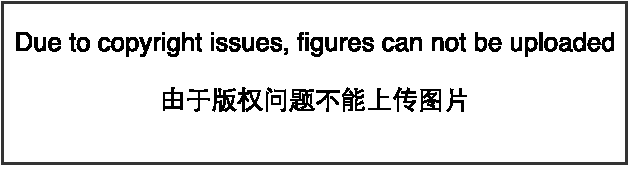
\includegraphics{figure.pdf}}
\else
\centerline{\includegraphics{Chapter11/figures/lr_color}}
\fi
\caption{TODO}
\label{fig:chap11_lr}
\end{figure}

调整学习率外的其他参数时,需要同时监测训练误差和测试误差,以判断您的模型是否过拟合或欠拟合,然后适当调整其容量。

如果训练集误差大于目标\gls{error_rate},那么你只能增加模型容量以改进模型。
如果您没有使用正则化,并且确信您的优化算法正确运行,那么您有必要添加更多层或更多\gls{hidden_unit}到网络中。
然而,令人遗憾的是,这增加了模型的计算代价。

% -- 417 --

如果测试集的误差大于目标\gls{error_rate},那么你可以采取两个办法。
测试误差是训练误差与训练误差和测试误差之间差距的总和。
寻找最佳的测试误差需要权衡这些数值。
当训练误差很小(因此容量较大),测试误差主要取决于训练误差和测试误差之间的差距时,通常神经网络效果最好。
你的目标是缩小这一差距,而不是训练误差的增速比差距减小得更快。
要减少差距,我们可以改变正则化超参数,以减少有效的模型容量,如添加\gls{dropout}或是权重衰减。
通常,最佳性能来自正则化比较好的大型模型,比如使用\gls{dropout}。

大部分超参数可以通过推理其是否增加或减少模型容量来设置。如表11.1所示部分实例。

手动调整超参数时,不要忘记最终目标:测试集上的优异性能。
加入正则化只是实现这个目标的一种方法。
只要训练误差低,随时都可以通过收集更多的训练数据来减少\gls{generalization_error}。
实践中保证成功的暴力方法就是不断提高模型模型和训练集的大小,直到解决问题。
这种做法当然增加了训练和推理的计算代价,所以只有在拥有适当资源的情况下才是可行的。
原则上,这种做法可能会因为优化难度提高而失败,但对于许多问题而言,优化似乎并没有成为一个显著的障碍,当然,前提是选择了合适的模型。

% -- 418 --

\subsection{自动超参数优化算法}
\label{sec:automatic_hyperparameter_optimization_algorithms}
理想的学习算法应该是只需要一个数据集,然后输出学习出的函数,而并不需要手动调整超参数。
一些流行的学习算法,如逻辑回归和支持向量机,流行的部分原因是只有一到两个需要调整的超参数,它们也能表现出不错的性能。
有时神经网络可以在只有少数需要调整的超参数时表现良好,但往往调整几十或者更多超参数会受益更明显。
当用户有一个很好的起点,例如由已经在相同类型的应用和架构上工作的其他人确定起点,或是用户已经在相似问题上探索了几个月甚至几年的神经网络超参数,那么手动调整超参数能有很好的效果。
然而,对于很多应用而言,这些起点都不可用。
在这些情况下,自动算法可以找到合适的超参数。

如果我们思考用户搜索学习算法合适超参数的方式,我们会意识到这其实是一种优化:
我们在试图寻找超参数来优化目标函数,例如验证误差,有时还会有一些约束(如训练时间,内存或识别时间的预算)。
因此,原则上有可能开发出封装学习算法的\firstgls{hyperparameter_optimization}算法,并选择其超参数,从而为用户隐藏学习算法的超参数。
令人遗憾的是,超参数优化算法往往有自己的超参数,如学习算法的每个超参数的值应该被探索的范围。
然而,这些次级超参数通常很容易选择,这是说,同一次级超参数能够很多问题上实现良好的性能。

\subsection{格点搜索}
\label{sec:grid_search}
当有三个或更少的超参数时,常见的超参数搜索方法是\firstgls{grid_search}。
对于每个超参数,用户选择一个较小的有限值集去探索。
然后,格点搜索算法训练为超参数笛卡尔乘积后的每个特定联合值训练模型。
挑选最好的验证集误差对应的超参数。
如图\ref{fig:chap11_grid_vs_random}所示超参数值的网络。

% -- 420 --

\begin{figure}[!htb]
\ifOpenSource
\centerline{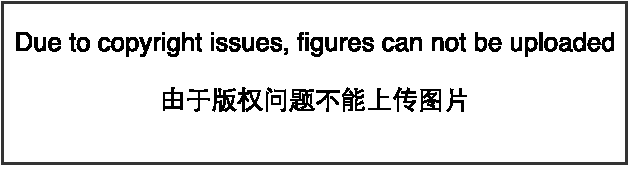
\includegraphics{figure.pdf}}
\else
\begin{tabular}{cc}
\includegraphics[width=0.4\textwidth]{Chapter11/figures/grid} &
\includegraphics[width=0.4\textwidth]{Chapter11/figures/random}
\end{tabular}
\fi
\caption{TODO}
\label{fig:chap11_grid_vs_random}
\end{figure}

应该如何选择搜索集合的值呢?
在超参数是数值(有序)的情况下,每个列表的最小和最大的元素可以基于先前相似实验的经验保守地挑选出来,以确保最优解非常可能在所选范围内。
通常,格点搜索大约会在\textbf{对数刻度}下挑选合适的值,例如,一个学习率的取值集合$\{0.1,0.01,10^{-3},10^{-4},10^{-5}\}$,或者隐单元数目的取值集合$\{50,100,200,500,1000,2000\}$。

通常重复进行格点搜索时,效果会最好。
例如,假设我们在集合$\{-1,0,1\}$上格点搜索超参数$\alpha$。
如果找到的最佳值是$1$,那么说明我们低估最优$\alpha$所在的范围,我们应该搜索范围,再次搜索$\alpha$,例如在集合$\{1,2,3\}$中搜索。
如果找到的最佳值是$0$,那么我们不妨通过细化搜索范围以改进估计,在集合$\{-.1,0,1\}$上进行格点搜索。

% -- 421 --

格点搜索带来的一个明显问题是,计算代价会随着超参数数量呈指数级增长。
如果有$m$个超参数,每个至多取$n$个值,那么训练和估计所需的试验数将是$O(n^m)$。
可以并行地进行实验,并且利用宽松的并行要求(不同搜索的机器之间几乎没有必要进行通信)。
令人遗憾的是,由于格点搜索指数级增长计算代价,即使并行也无法提供令人满意的计算能力。


\subsection{随机搜索}
\label{sec:random_search}
幸运的是,有一个格点搜索的替代方法,并且其编程简单,使用更方便,能更快地收敛到超参数的良好值:随机搜索\citep{Bergstra+Bengio-2012-small}。

随机搜索过程如下。
首先,我们定义每个超参数定义一个边缘分布,例如,伯努利分布或分类分布(对应着二元超参数或离散超参数),或者对数尺度上的均匀分布(对应着正实值超参数)。
例如,
\begin{align}
	\texttt{log\_learning\_rate} &\sim u(-1, -5), \\
	\texttt{learning\_rate} &= 10^{\texttt{log\_learning\_rate}},
\end{align}
其中,$u(a,b)$表示区间$(a,b)$上均匀采样的样本。
类似地,$\texttt{log\_number\_of\_hidden\_units}$可能表示采样自$u(\log(50), \log(2000))$。

和格点搜索的情况不同,我们\emph{不应该离散化}超参数的值,从而我们可以去探索一个更大集合的值,而不产生额外的计算代价。
实际上,如图11.2所示,当有几个超参数对\gls{performance_metrics}没有很强的影响时,随机搜索指数级高效于格点搜索。
\cite{Bergstra+Bengio-2012-small}进行了详细的研究,发现随机搜索减小验证集误差比格点搜索要快得多(就每个模型运行的试验数而言)。

与格点搜索一样,可以经常重复运行不同版本的随机搜索,以基于前一次运行的结果改进下一次搜索。

随机搜索能比格点搜索更快地找到好解的原因是,没有浪费的实验,不像格点搜索有时会遇到一个超参数的两个值(给定其他超参数值不变)会给出相同结果的情况。
在格点搜索中,其他超参数将在这两次实验中拥有相同的值,而在随机搜索中,它们通常会具有不同的值。
因此,如果这两个值的变化不能勉强使验证集误差有明显区别的话,格点搜索没有必要重复两个等价的实验,而随机搜索仍然会对其他超参数进行两次独立地探索。

% -- 422 --

\subsection{基于模型的超参数优化}
\label{sec:model_based_hyperparameter_optimization}
良好超参数的搜索可以转换为一个优化问题。
决策变量是超参数。
优化的目标是使用这些超参数训练结果的验证集误差。
在简化的设定下,可以计算验证集上可导误差关于超参数的导数,然后我们遵循这个导数更新\citep{bengio:1999:snowbird,bengio-hyper-NC00,maclaurin2015gradient}。
令人遗憾的是,在大多数实际设定中,这个梯度是不可用的。这要么是因为其高计算代价和存储成本,要么是因为验证集误差在超参数上具有本质的不可导,例如超参数是离散值的情况。

为了弥补导数这一不足,我们可以对验证集误差建模,然后通过优化该模型来提出新的超参数猜想。
大部分基于模型的超参数搜索算法都使用贝叶斯回归模型来估计每个超参数的验证集误差期望,和该期望的不确定性。
因此,优化涉及到探索(探索高度不确定的超参数,可能有重大效果提升,也可能效果很差)和使用(使用已经确信效果不错的超参数---通常是先前非常熟悉的超参数)之间的权衡。
关于超参数优化,现在的方法还有Spearmint\citep{Snoek+al-NIPS2012-small},TPE\citep{Bergstra+al-NIPS2011}和SMAC\citep{hutter+hoos+leyton+brown:2011}。

目前,我们无法明确建议贝叶斯超参数优化是一个能够实现更好\gls{DL}结果或是能够事半功倍的工具。
贝叶斯超参数优化有时表现得像人类专家,有时还能更好,但在有些问题上又会发生灾难性的故障。
看看它是否适用于一个特定的问题是值得尝试的,但目前该方法还不够成熟或可靠。
就像所说的那样,超参数优化是一个重要的研究领域,通常主要受\gls{DL}所需驱动,但是它不仅能贡献于整个\gls{ML}领域,还能有益于一般的工程学。

% -- 423 --

比随机搜索更复杂的大部分超参数优化算法的一个共同缺点是在它们能够从实验中提取任何信息之前,它们需要运行完整的训练实验。
相比于人类实践者手动搜索,对于实验早期可以收集多少信息,这是相当低效的,因为手动搜索收集通常可以很早判断出某组超参数是否是完全病态的。
\cite{swersky2014freeze}提出了一个可以维护多个实验的早期版本算法。
在不同的时间点,超参数优化算法可以选择开启一个新实验,“冻结”正在运行但希望不大的实验,或是“解冻”并恢复早期被冻结的,但现在根据更多信息后又有希望的实验。

\section{调试技巧}
\label{sec:debugging_strategies}
当一个\gls{ML}系统效果不好时,通常很难判断效果不好的来源是算法本身,还是算法实现中的错误。
由于各种原因,\gls{ML}系统很难调试。

在大多数情况下,我们不能提前知道算法的预期行为。
事实上,使用\gls{ML}的整个出发点是,它会发现一些我们自己无法发现的有用行为。
如果我们在一个\emph{新}的分类任务上训练一个神经网络,它达到$5\%$的测试误差,我们没法直接知道这是期望的结果,还是次优的结果。

另一个难点是,大部分\gls{ML}模型有多个自适应的部分。
如果一个部分失效了,其他部分仍然可以自适应,并获得大致可接受的性能。
例如,假设我们正在训练多层神经网络,其中参数为权重$\MW$和\gls{bias_aff}$\Vb$。
进一步假设,我们单独手动实现了每个参数的梯度下降规则。
而我们在偏置更新时犯了一个错误:
\begin{equation}
	\Vb \leftarrow \Vb - \alpha,
\end{equation}
其中$\alpha$是学习率。
这个错误更新没有使用梯度。
它会导致偏置在整个学习中不断变为负值,而这显然不是任何一个合理学习算法的正确实现。
然而只是检查模型的输出,该错误可能并不是显而易见的。
根据输入的分布,权重可能可以自适应地补偿负的偏置。

% -- 424 --

大部分神经网络的调试技巧都是旨在解决这两个难题的一个或两个。
要么我们设计一种简单的情况,实际上可以预见正确的结果,要么我们设计一个测试,单独检查神经网络实现的一部分。

一些重要的调试检测包括以下这些。

\emph{可视化模型的行为}:
当训练模型来检测图像中的物体时,查看一些模型检测到部分重叠的图像。
在训练语音生成模型时,试听一些生成的语音样本。
这似乎是显而易见的,但在实际中很容易只注意量化\gls{performance_metrics},如精度或对数似然。
直接观察\gls{ML}模型运行任务,有助于确定其达到的量化性能数据是否看上去合理。
评估错误可能是最具破坏性的错误之一,因为它们会使你在系统出问题时误以为系统运行良好。

\emph{可视化最严重的错误}:
大多数模型能够输出运行任务时的某种置信度量。
例如,基于\gls{softmax}输出层的分类器给每个类分配一个概率。
因此,分配给最有可能的类的概率给出了模型在其分类决定上的置信估计值。
通常,这些值上的最大似然训练结果高估了正确预测的准确概率,
但是由于实际上模型下的较小概率不太可能对应着正确的标签,因此它们在一定意义上还是有些用的。
通过查看训练集中很难正确建模的样本,通常可以发现该数据预处理或者标记方式的问题。
例如,街景\gls{transcription_system}原本有个问题是,地址号码检测系统会将图像裁剪得过于紧密,而省略掉了一些数字。
然后转录网络会分配非常低的概率给这些图像的正确答案。
将图像排序,确定置信度最高的错误,显示系统的裁剪有问题。
修改检测系统裁剪更宽的图像,从而使整个系统获得更好的性能,但是转录网络需要能够处理地址号码中位置和范围更大的变化。

\emph{使用训练和测试误差检测软件}:
往往很难确定底层软件是否是正确实现。
训练和测试误差能够提供一些线索。
如果训练误差较低,但是测试误差很高,那么很有可能训练过程是在正常运行,但模型由于算法原因过拟合了。
另一种可能是,测试误差没有被正确地度量,可能是由于训练后保存模型再重载去度量测试集时出现的问题,或者是因为测试数据和训练数据预处理的方式不同。
如果训练和测试误差都很高,那么很难确定是软件缺陷,还是模型由于算法原因欠拟合。
这种情况需要进一步的测试,如下面所述。

% -- 425 --

\emph{拟合小数据集}:
如果你在训练集上有很大的误差,确定问题是否是由于欠拟合,还是由于软件缺陷。
通常,即使是小模型也可以保证很好地拟合一个足够小的数据集。
例如,只有一个样本的分类数据可以通过正确设置输出层的偏置来拟合。
通常,如果你不能训练一个分类器来正确标注一个单独的样本,或是一个自编码来成功地精准再现一个单独的样本,或是一个生成模型来一致地生成一个单独的样本,那么很有可能是由于软件缺陷阻止训练集上的成功优化。
此测试可以扩展到只有少量样本的小数据集上。

\emph{比较反向传播导数和数值导数}:
如果您正在使用一个需要您实现梯度计算的软件框架,或者您在添加一个新操作到求导库中,必须定义它的\text{bprop}方法,那么常见的错误原因是没能正确执行这一梯度表达。
验证这些求导正确的一种方法是比较实现的自动求导和\firstgls{finite_difference}计算的导数。
因为
\begin{equation}
	f'(x) = \lim_{\epsilon \to 0} \frac{f(x+\epsilon) - f(x)}{\epsilon},
\end{equation}
我们可以使用小的,有限的$\epsilon$近似导数:
\begin{equation}
	f'(x) \approx \frac{f(x+\epsilon) - f(x)}{\epsilon}.
\end{equation}
我们可以使用\firstgls{centered_difference}提高近似的精度:
\begin{equation}
	f'(x) \approx \frac{ f(x+\frac{1}{2}\epsilon) - f(x-\frac{1}{2}\epsilon) }{\epsilon}.
\end{equation}
扰动大小$\epsilon$必须足够大,以确保该扰动不会由于数值计算的有限精度问题向下近似太多。

% -- 426 --

通常,我们会测试矢量值函数$g:\SetR^m \to \SetR^n$的梯度或雅可比矩阵。
令人遗憾的是,\gls{finite_difference}只允许我们每次计算一个导数。
我们既可以运行\gls{finite_difference}$mn$次评估$g$的所有偏导数,又可以将该测试应用于一个输入输出都是$g$的随机投影的新函数。
例如,我们可以应用导数实现的测试于函数$f(x) = \Vu^T g(\Vv x)$,其中$\Vu$和$\Vv$是随机向量。
正确计算$f'(x)$要求能够正确地通过$g$反向传播,但是使用有限差分能够很有效地计算,因为$f$只有一个输入和一个输出。
在多个$\Vu$值和$\Vv$值上重复这个测试通常是个好主意,可以减少测试忽略了垂直于随机投影的几率。


如果可以在复数上进行数值计算,那么使用复数作为函数的输入能有非常高效的数值方法估算梯度\citep{Squire+Trapp-1998}。
该方法基于如下观察
\begin{align}
	f(x + i\epsilon) &= f(x) + i\epsilon f'(x) + O(\epsilon^2) ,\\
	\text{real}( f(x+i\epsilon) ) &= f(x) + O(\epsilon^2), \quad \text{image}( \frac{f(x+i\epsilon)}{ \epsilon } ) = f'(x) + O(\epsilon^2),
\end{align}
其中$i=\sqrt{-1}$。
和上面的实值情况不同,这里不存在$f$在不同点上计算差分时的消除影响。
因此我们可以使用很小的$\epsilon$,比如$\epsilon = 10^{-150}$,其中误差$O(\epsilon^2)$对所有实用目标都是微不足道的。


\emph{监控激励函数值和梯度的直方图}:
可视化神经网络在大量训练迭代后(也许是每个迭代)收集到的激励函数值和梯度的统计数据往往是有用的。
\gls{hidden_unit}的预激励值可以告诉我们该单元是否饱和,或者它们平常的状态如何。
例如,对于整流器,它们多久关一次?是否有单元一直关闭?
对于双曲正切单元而言,预激励绝对值的平均值可以告诉我们该单元的饱和程度。
在深度网络中,传播的梯度可以快速增长或快速消失,优化可能会受到阻碍。
最后,比较参数梯度和参数的量值也是有帮助的。
正如\citep{Bottou-DLSS2015}的建议,我们希望参数在一个\gls{minibatch}更新中变化的幅度是像参数量值$1\%$这样的大小,而不是$50\%$或者$0.001\%$(这会导致参数移动得太慢)。
也有可能是某些参数以良好的步长移动,而另一些停滞。
如果数据是稀疏的(比如自然语言),有些参数可能很少更新,检测它们变化时应该记住这一点。

% -- 427 --

最后,许多\gls{DL}算法为每一步产生的结果提供了某种保证。
例如,在第三部分,我们将看到一些使用代数解决优化问题的近似推理算法。
通常,这些可以通过测试它们的每个担保来调试。
某些优化算法提供的保证包括,目标函数值在算法的迭代步中不会增加,某些变量的导数在算法的每一步中都是零,所有变量的导数都会收敛到零。
通常,由于舍入误差,这些条件不会在数字计算机上完全成立,因此调试测试应该包含一些允差参数。

\section{示例:多位数字识别}
\label{sec:example_multi_digit_number_recognition}
为了\gls{end_to_end}地说明如何在实践中应用我们的设计方法,我们从设计\gls{DL}组件的角度出发,简单地介绍下街景\gls{transcription_system}。
显然,整个系统的许多其他组件,如街景车,数据库设施,等等,也是极其重要的。

从\gls{ML}任务的视角出发,首先这个过程要采集数据。
街景车收集原始数据,然后操作员手动提供标签。
转录任务开始前有大量的数据处理工作,包括在转录前使用其他\gls{ML}技术\emph{探测}房屋号码。

转录项目开始于\gls{performance_metrics}的选择,及这些度量的期望。
一个重要的总原则是度量的选择要符合项目的业务目标。
因为地图只有是高精度时才有用,所以为这个项目设置高精度的要求非常重要。
具体地,目标是达到人类水平,$98\%$的准确率。
这种程度的精度并不是总能达到。
为了达到这个级别的准确性,街景\gls{transcription_system}牺牲了\gls{coverage}。
因此在保持精度$98\%$的情况下,\gls{coverage}成了这个项目优化的主要\gls{performance_metrics}。
随着卷积网络的改进,能够降低网络拒绝转录输入的置信度阈值,最终超出了\gls{coverage}$95\%$的目标。

% -- 428 --

在选择量化目标后,我们推荐方法的下一步是要快速建立一个合理的基准系统。
对于视觉任务而言,这意味着带有\gls{ReLU}的卷积网络。
转录项目开始于这样一个模型。
当时,使用卷积网络输出预测序列并不常见。
开始于一个尽可能简单的基准,该模型输出层的第一个实现包含$n$个不同的\gls{softmax_unit}来预测$n$个字符的序列。
这些\gls{softmax_unit}和分类任务时的训练完全一样,每个\gls{softmax_unit}被单独训练。


我们推荐的方法是反复细化这些基准,并测试每个变化是否都有改进。
街景\gls{transcription_system}的第一个变化受激励于\gls{coverage}指标的理论理解和数据的结构。
具体地,当输出序列的概率低于某个值$t$,$p(\Vy|\Vx) < t$时,网络拒绝为输入$\Vx$分类。
最初,$p(\Vy|\Vx)$的定义是临时的,简单地将所有\gls{softmax}输出乘在一起。
这促使了能够真正计算出合理对数似然的特定输出层和损失函数的发展。
这种方法使得样本拒绝机制发挥得更有效。


此时,\gls{coverage}仍低于$90\%$,但该方法没有明显的理论问题了。
因此,我们的方法建议综合训练集和测试集性能,以确定问题是否是欠拟合或过拟合。
在这种情况下,训练和测试集误差几乎是一样的。
事实上,这个项目进行得如此顺利的主要原因是有数以千万计的标识样本数据集可用。
因为训练和测试集的误差是如此相似,这表明要么是这个问题欠拟合,要么是训练数据的问题。
我们推荐的调试技巧之一是可视化模型最糟糕的错误。
在这种情况下,这意味着可视化不正确而模型给了最高置信度的训练集转录。
结果显示,主要是输入图像裁剪得太紧,有些和地址相关的数字被裁剪操作除去了。
例如,地址“1849”的图片可能裁切得太紧,只剩下“849”是可见的。
花费几周改进负责确定裁剪区域的地址号码检测系统的精度,或许可以解决这个问题。
与之不同,该项目团队采取了更实际的决定,简单地系统性扩大裁剪区域的宽度大于地址号码检测系统预测的区域。
这种单一改变给\gls{transcription_system}的\gls{coverage}增加了$10$个百分点。

% -- 429 --

最后,性能提升的最后几个百分点来自调整超参数。
这主要包括在保持一些计算代价限制的同时加大模型的规模。
因为训练和测试误差几乎保持相等,所以明确表明性能不足是由于欠拟合造成的,和数据集本身也存在一些问题。


总体来说,转录项目是非常成功的,可以比人工速度更快,代价更低地转录数以亿计的地址。

我们希望本章中介绍的设计原则能带来更多其他类似的成功。

% -- 430 --
